
% !TeX root = ../book.tex
% !TeX spellcheck = fr_FR
% !TeX encoding = ISO-8859-1

\section{Rappel � la petite bande}

Voil� encore un point qui se pr�sente tr�s fr�quemment. On peut aussi le
rencontrer le long de la petite bande ou bien dans le champ, la 3
n'�tant pas proche d'une bande.

Figure 1 : c'est le cas la plus courant. C'est un r�tro angle droit
appuy�, effet favorable. La 1 touche une bande ou parfois deux et la 2
se rappelle par trois bandes. Si l'inclinaison est trop faible sur la
grande bande de la direction 1-2, il sera peut-�tre pr�f�rable
d'attaquer la 2 plus grosse pour assurer sa rentr�e dans le chapeau. Il
conviendra alors de jouer un peu plus haut sur la 1 tout en restant sous
le milieu de la hauteur. Dans le m�me ordre d'id�e, si l'inclinaison 1-2
sur la grande bande semble trop imposante, il sera pr�f�rable d'attaquer
la 2 moins grosse avec une prise de la 1 un peu plus basse et �a,
toujours pour s'assurer la rentr�e au chapeau.

Figure 2 : L'inclinaison 1-2 sur la grande bande est faible et un 1B tel
que pour la figure 2 enverrait la 2 dans le coin oppos� loin de la 3 et
un r�tro direct ne permettrait pas un retour de la 2. On peut encore
tenter un 1B mais sans effet, voire effet contraire. La 2, faiblement
�cart�e de la grande bande, ne poss�de alors aucun effet qui
favoriserait son �loignement. La tentative avec effet contraire est
cependant assez difficile et une bonne habitude sera n�cessaire.

Remarques :

Plut�t que de risquer de voir la 3 � soulev�e � par la deuxi�me bande
de la 2, il sera souvent pr�f�rable de tenter un 1B sec qui �crasera la 3 sur la petite bande,
l'emp�chant de se sauver du chapeau. La 3 se trouvant dans le tiers
central de la petite bande, il conviendra avant l'essai, de bien estimer
le retour de la 2. Il serait dommage que le 2 rentre au coin derri�re le
jeu pendant que vous restez au milieu de la bande avec la 3. Enfin si la
taille du point d�passe un tiers de la table, la r�alisation devient
difficile et les retours plus al�atoires.

A l'entra�nement, il sera int�ressant d'essayer le bon effet, le sans
effet et l'effet contraire sans changer la position des billes au
d�part. Vous vous rendrez compte tr�s facilement des diff�rents
r�sultats et cela vous aidera dans vos choix futurs.

\begin{figure}[htb]
	\centering
	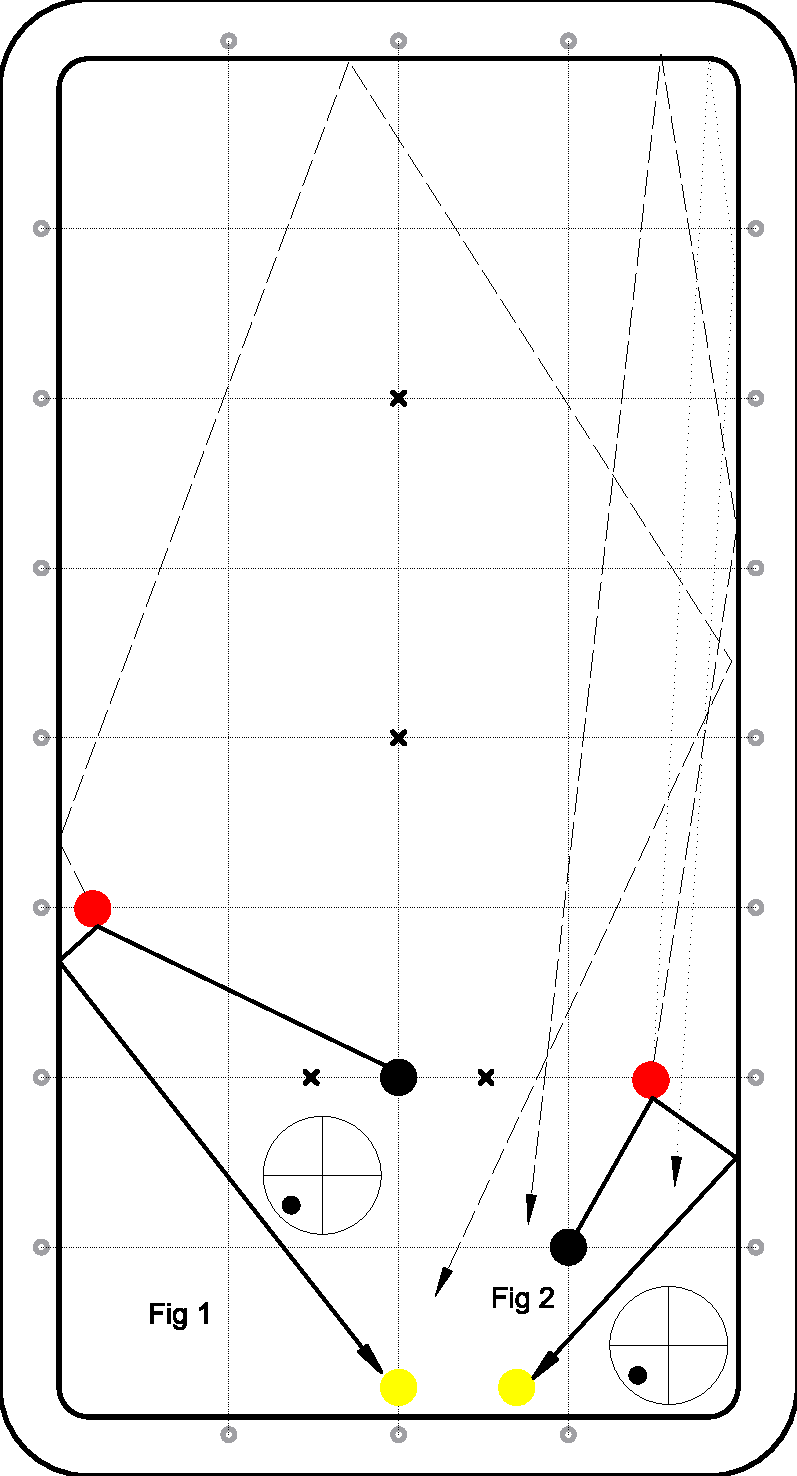
\includegraphics[width=0.85\linewidth]{B/imagesB/B08-01.pdf}
	\caption{Rappel � la petite bande}
	\label{fig:B08-1}
\end{figure}

\clearpage
